%!TEX root = ../dokumentation.tex

\chapter{Stand der Technik}
Die Verwendung von Virtual Reality in der Forschung setzt sich immer weiter durch. Vor allem die Digitalisierung der Versuchsumgebung bringt einige enorme Vorteile für die Forschung mit sich. Beispielsweise können Versuche in \ac{VR} beliebig oft mit genau dem gleichen Aufbau wiederholt werden. \ac{VR} mit Eye-Tracking zu koppeln bietet daher sehr viele interessante Möglichkeiten \cite{Clay_Koenig_Koenig_2019}. Im Folgenden werden aktuelle Erkenntnisse zu \ac{VR} in Kombination mit Eye-Tracking vorgestellt.

\section{Verwendung von Eye-Tracking in VR}
Eye-Tracking kann in Verbindung mit \ac{VR} in vielen unterschiedlichen Bereichen eingesetzt werden \cite{Clay_Koenig_Koenig_2019}. Diese verschiedenen Gebiete werden in den folgenden Abschnitten näher betrachtet.
\subsection{Erforschung von Blickverhalten}
Mittels Eye-Tracking lässt sich sehr gut feststellen, worauf ein Nutzer seine Aufmerksamkeit richtet. Dies kann unter anderem in Marketing \cite{C.Wang.2019} oder anderen Gebieten eingesetzt werden, wo die wichtigsten Informationen möglichst präsent gezeigt werden sollen. 
Ein Beispiel für die Anwendung in der Forschung zum Blickverhalten ist die Forschung von \citeauthor{P.Tian.2019}, in der das Blickverhalten von Probanden in einer \ac{VR} Umgebung eines brennenden Raumes analysiert wurde. Da ein brennender Raum in echt keine wiederholbaren Forschungen erlauben würde, ganz abgesehen von der Gefährdung der Probanden, bietet sich hier die Forschung mit \ac{VR} an. Dadurch können Versuche mit mehreren Probanden in genau dem gleichen Umfeld mit genauen Daten durchgeführt werden. Ziel der Studie war es, eine Evaluierung der Fluchtwege in vorgefertigten Szenarien zu ermöglichen. Durch die Analyse der Blickdaten ist es möglich zu erkennen, wo der Nutzer zu welchem Zeitpunkt hinschaut. Dadurch kann festgestellt werden, ob Hinweise zum nächsten Fluchtweg schnell gefunden werden, und wenn nicht, wie Hinweise besser platziert werden können. Die Studie kam zu dem Ergebnis, dass mit dieser Methode eine bessere Evaluierung der Fluchtwege, vor allem in Gefahrensituationen möglich ist. \cite{P.Tian.2019}

Ein weiteres Beispiel zur Erforschung des Blickverhaltens bietet die Studie von \citeauthor{K.Hotta.2019}. Hier wurde das aktive Sichtfeld der Probanden untersucht, indem ein Lichtreiz im Sichtfeld des Probanden ausgelöst wird und der Proband reagiert, sobald er den Lichtreiz wahr nimmt. Das Ziel der Studie ist es, die bisherigen Forschungen, die zu diesem Thema betrieben wurden, zu verbessern, indem der Versuch in \ac{VR} in Verbindung mit Eye-Tracking übertragen wird. Durch die Übertragung in \ac{VR} ergibt sich der Vorteil, dass der Kopf nicht mehr fixiert werden muss, da das Display mit \ac{VR} am Kopf des Probanden fixiert ist. Somit sind freie Kopfbewegungen möglich, da der Bildschirm sich entsprechend mitbewegt. Des weiteren bietet der Eye-Tracker einen enormen Mehrwert, da Reaktionen der Augen direkt aufgezeichnet werden. In den vorherigen Studien musste der Proband aktiv angeben, wann er den Reiz wahrgenommen hat. Damit war es den Forschern möglich, die Zeit pro Versuch von rund 30 Minuten im vorherigen Versuchsaufbau auf fünf Minuten zu reduzieren und dabei verlässlichere Ergebnisse zu produzieren.\cite{K.Hotta.2019}

\subsection{Foveated rendering}
\label{section:foveated}
Der treibende Faktor hinter der Entwicklung von \ac{VR} ist der Gaming Markt. Das ist daran zu erkennen, dass alle großen Firmen in der \ac{VR}-Branche aus der Gaming-Branche kommen, oder über Umwege mit ihr zu tun haben. Die Geräte von HTC beispielsweise sind in Zusammenarbeit mit dem Videospiel Publisher Valve entwickelt worden, der mit Steam\ac{VR}-seine eigene Schnittstelle für \ac{VR} Anwendungen anbietet (vgl. \autoref{section:steamvr}) \cite{ViveProduct}. Valve hat mit der Valve Index mittlerweile auch ein eigenes \ac{VR}-Headset auf den Markt gebracht \cite{Index}. Der Hersteller Oculus VR, eine Tochterfirma von Facebook und einer der Pioniere der \ac{VR}-Szene, hat seine erste Brille mit dem Hauptziel, \ac{VR}-Gaming für die breite Masse zugänglich zu machen, auf den Markt gebracht \cite{OculusKickstarter}. Jedoch ist \ac{VR} momentan noch sehr Ressourcenintensiv. Ein Blick auf die Systemanforderungen der Hersteller zeigt, dass meist ein sehr starker Computer, vor allem mit starker Grafikkarte benötigt wird, um ein angenehmes \ac{VR} Erlebnis zu erzielen \cite{Lang.2019}. Die enorme Rechenkraft, die benötigt wird, um ein \ac{VR} Headset zu betreiben, kann allerdings reduziert werden. Hierfür wird das sogenannte Foveated Rendering genutzt. Dabei wird Eye-Tracking genutzt, um den Bereich des Bildes zu bestimmen, der vom Nutzer gerade fixiert wird (Region of Interest). Dieser Bereich wird dann in der vollen Auflösung berechnet, während der restliche Teil des Bildes in einem Bruchteil der tatsächlichen Auflösung berechnet wird\cite{Albert.2017}.

\begin{figure}
	\centering
	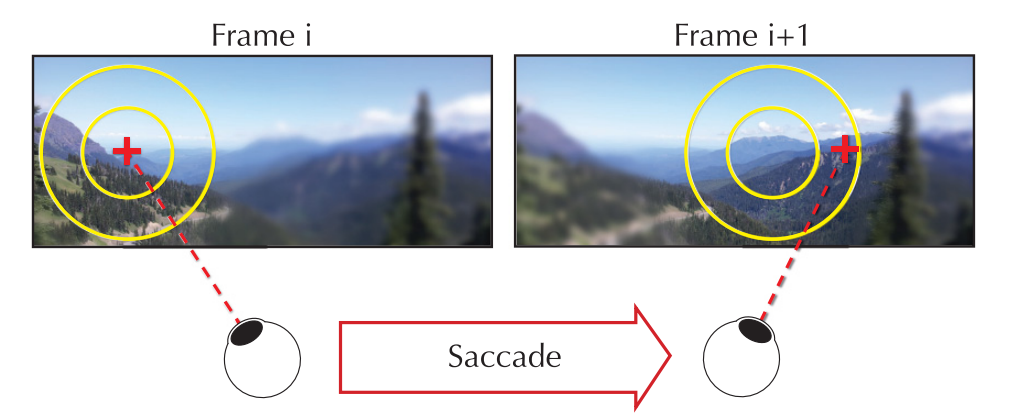
\includegraphics[width=\linewidth]{foveated_rendering}
	\caption[Foveated Rendering Beispiel]{Foveated Rendering Beispiel \cite{Albert.2017}}
	\label{fig:foveated}
\end{figure}

In der \autoref{fig:foveated} ist schemenhaft zu sehen, wie Foveated Rendering funktioniert. Der Bereich, der fokussiert wird, wird scharf dargestellt. Der Bereich rund um den fokussierten Bereich wird ebenfalls scharf dargestellt, allerdings nicht so scharf wie der Hauptbereich.  Der restliche Bereich wird unscharf dargestellt. Da der Nutzer diesen Bereich nicht aktiv anschaut, fällt auch die geringere Auflösung nicht auf. Während einer Sakkade werden Objekte vom Auge nicht komplett scharf wahrgenommen, weshalb es für den Nutzer nicht spürbar ist, dass ein Bereich des Bildes nicht scharf dargestellt wird. Die Zeit, bis das Auge sich auf einen neuen Punkt fixiert hat ist ausreichend, um das Bild in diesem Bereich scharf zu stellen, so dass dem Nutzer der Einsatz von Foveated Rendering nicht auffällt \cite{Albert.2017}. Der Einsatz von Foveated Rendering kann die Last auf den Computer deutlich reduzieren. In ersten Versuchen ist eine Erhöhung der Bilder pro Sekunde (Frames per Second, fps) von 10-15 Prozent beobachtbar gewesen. \cite{H.Kim.2018}

\subsection{Interaktionen}
Eye-Tracking kann in \ac{VR} auch für Interaktionen genutzt werden. Dies hat vor allem für körperlich benachteiligte Menschen einen enormen Vorteil, da diese meist nicht die herkömmlichen Steuermöglichkeiten verwenden können. Ebenso erhöht eine derartige Steuerung die Immersion in die \ac{VR}-Welt, was für eine noch bessere Simulationserfahrung sorgt. Eine genauere Beschreibung der unterschiedlichen Arten des Eye-Trackings und der Interaktionsmöglichkeiten hiermit sind in Abschnitt \ref{eyetrackingVR} zu finden.

\section{Steuermöglichkeiten in VR}
Mit einer Umgebung in \ac{VR} kann auf verschiedenste Arten interagiert werden. In diesem Abschnitt werden die relevantesten Interaktionsmöglichkeiten vorgestellt. Die Grundlage hierfür ist ein \ac{VR}-System in Verbindung mit einem Computer. Eigenständige Systeme, wie Google Cardboard, Oculus Quest oder PlayStation \ac{VR} werden nicht beachtet.

\subsection{Herkömmliche Steuerarten}
Bei den herkömmlichen Eingabegeräten ist eine Unterteilung in \ac{VR}-Eingabgeräte und Non-\ac{VR}-Eingabegeräte möglich. \ac{VR}-Eingabegeräte sind beispielsweise die Controller der HTC Vive (vgl. \autoref{section:controller}). Non-\ac{VR}-Eingabegeräte sind Geräte, wie Maus, Tastatur oder Gamepad.
Da die Nutzung eines \ac{VR}-Systems meist mit einem Computer verbunden ist, ist die Steuerung über die herkömmlichen Eingabegeräte auch hier möglich. Die Nutzung einer Tastatur, Maus oder eines Gamepads, wie etwa einem Xbox-Controller ist hier ohne Probleme möglich und wird teilweise auch verwendet. Allerdings ist diese Steuerart nicht sehr weit verbreitet, da \ac{VR}-Systeme meist keine Unterstützung für das Darstellen dieser Objekte in \ac{VR} anbieten. Dadurch ist es für den Nutzer nicht möglich, das Gerät zu sehen, was eine Bedienung erschweren kann. Nichtsdestotrotz gibt es Ansätze, diese Steuermöglichkeiten zu verwenden. Beispielsweise ist auf GitHub eine Modifizierung für das Spiel Grand Theft Auto V veröffentlicht worden, die es ermöglicht, das Spiel in \ac{VR} mit einem Xbox-Controller zu spielen \cite{Werner.2020}. Das Rennspiel Project Cars hat ebenso eine \ac{VR}-Unterstützung eingebaut. Hier wird zur Steuerung ein Lenkrad empfohlen, welches man als Eingabegerät an den Computer anschließen kann \cite{projCars}. Diese beiden Steuerarten sind von den herkömmlichen Non-\ac{VR}-Eingabegeräten am meisten geeignet, da der Nutzer, im Gegensatz zu Tastatur und Maus, die Hände immer am Eingabegerät hat und es somit nicht relevant ist, dass die Position dieser Geräte in \ac{VR} angezeigt wird.

Die herkömmlichen \ac{VR}-Eingabegeräte sind zwei Controller, welche in beiden Händen gehalten werden. Die Controller haben Erkennungsmerkmale, sodass die Position vom Tracking-System erfasst werden kann. Die Steuerung in den \ac{VR}-Umgebungen findet meist nach dem Laserpointer Prinzip statt (vgl. \autoref{section:controller}). Das bedeutet, dass ein Laserpointer in der virtuellen Umgebung vom Controller ausgeht und mit dem Betätigen des Triggers an der Unterseite bestätigt werden kann. Ebenso gibt es Implementierungen, bei denen die Controller wie Hände genutzt werden. Hier bieten die Controller der Valve Index einen Vorteil, da diese die Position der Finger am Controller wahrnehmen und die Handposition so in die virtuelle Welt übertragen \cite{Index.Controller}.

\subsection{Hand-Tracking}
Um die Immersion in \ac{VR} weiter voranzutreiben, ist Hand-Tracking, ohne einen Controller, ein Ansatz, um Interaktionen in \ac{VR} mit den Händen auf natürliche Weise zu erlauben. 
Technisch gibt es grob zwei Ansätze für Hand-Tracking. Einerseits gibt es (Infrarot-)Kamerabasierte Systeme, wie Leap Motion \cite{Leap.2014}, andererseits gibt es Ansätze über sogenannte Data Gloves \cite{S.Lee.2017}. Die Kamerabasierten Systeme Nutzen das Kamerabild, um die Handposition zu erkennen und in \ac{VR} einzubringen. Bei den Data-Gloves werden Sensoren an den Händen angebracht, die die Bewegungen der Hände wahrnehmen und in Modellierungen der Hände übertragen. 

\subsection{Eye-Tracking und Head-Tracking}
\label{eyetrackingVR}
Eye-Tracking in \ac{VR} ist für gewöhnlich kamerabasiert. Das bedeutet, dass die Position der Pupillen mit Kameras bestimmt wird und daraus die Blickrichtung abgeleitet wird (vgl. \autoref{section:eyetracking})\cite{Blake.2013}. Der Ansatz, der von \citeauthor{D.Kumar.2016} in ihrer Untersuchung zu Eye-Tracking verfolgt wurde, ist jedoch nicht kamerabasiert, sondern basiert auf einem Elektrookulogramm (\ac{EOG}). Dabei werden Elektroden rund um die Augen am Nutzer befästigt und die Augenbewegungen anhand der elektrischen Signale zu den Muskeln, welche für die Bewegung der Augen zuständig sind, aufgezeichnet. Die Forscher haben diesen Ansatz gewählt, um die Steuerung einer \ac{VR}-Portierung eines Spiels bereitzustellen. Die Probanden der Studie konnten mit Blickrichtungen eine Spielfigur eine Strecke entlanglaufen lassen. Die Forscher kamen zu dem Schluss, das eine \ac{EOG}-basierte Steuerung eine ungefährliche und immersive Steuermöglichkeit in \ac{VR} ist. \cite{D.Kumar.2016}

Eine weitere Untersuchung zu Eye-Tracking als Steuermöglichkeit wurde von \citeauthor{Pai.2019} durchgeführt. Dabei wurden verschiedene Eingabemethoden verglichen. Zu diesen Eingabemethoden zählten HTC Vive Controller, Xbox Controller, Eye-Tracking mit Verweilen (dwelling) zum Auswählen des Objekts und Eye-Tracking mit einer Anspannung im Unterarm, welche über Elektroden aufgezeichnet wird, zum Auswählen des Objekts. In der Studie hat sich Eye-Tracking in Kombination mit Anspannungen im Unterarm als am effektivsten herausgestellt. \cite{Pai.2019} Diese Studie ist für diese Arbeit besonders relevant, da die zentrale Frage eine sehr ähnliche ist. Sowohl in der Arbeit von \citeauthor{Pai.2019}, als auch in dieser Arbeit wird Eye-Tracking mit anderen Steuermöglichkeiten verglichen.

Eine weitere Art der Steuerung über den Blick ist das Head-Tracking. Hier besteht der große Vorteil, dass nicht die Augen, sondern die Kopfposition die Steuerung ermöglichen. Das bedeutet zwar, dass immer angenommen wird, der Nutzer schaut direkt voraus, allerdings ist das meistens der Fall. Somit kann über Head-Tracking, welches standardmäßig in jedem \ac{VR}-System integriert ist, eine Steuerung ohne externe Hardware ermöglicht werden, die einer Blicksteuerung ähnelt. In einer Studie von \citeauthor{R.Atienza.2016} wurde getestet, ob der sogenannte \glqq Head Gaze\grqq{} eine Steuermöglichkeit darstellt. Dabei wurden mehrere Spiele abgeändert, sodass Kopfbewegungen als Eingabe wahrgenommen werden. Die neue Eingabemethode wurde von den Probanden als immersiv wahrgenommen, allerdings war die neue Steuerart auf Dauer auch anstrengend. Allerdings stellen diese Ergebnisse vor allem für den \ac{VR}-Markt auf Smartphone Basis, wie etwa Google Cardboard und Samsung Gear VR, eine neue Steuermöglichkeit dar, die ohne weitere Hardware implementiert werden kann. \cite{R.Atienza.2016}

\section{Bisherige Erkenntnisse zu Eye-Tracking als Steuerung im Vergleich zu anderen Steuermöglichkeiten}
Bisherige Untersuchungen zu Eye-Tracking als Steuerung haben größtenteils positive Ergebnisse vorgebracht. So ist zum Beispiel in den Versuchen von \citeauthor{Pai.2019} herausgekommen, dass Eye-Tracking die effektivste von mehreren Methoden zum Auswählen bestimmter Objekte ist. Dabei war Eye-Tracking effektiver, als der Einsatz von HTC Vive Controllern und anderen Steuermöglichkeiten. Dies wurde anhand eines Aufbaus festgestellt, der sich an Fitts' Gesetz orientiert und in einem Spiel, in dem der Proband mit einer Waffe zielen und schießen muss. \cite{Pai.2019}

Auch andere Studien, wie die von \citeauthor{D.Kumar.2016} oder \citeauthor{R.Atienza.2016} zeigen, dass Eye-Tracking eine gute Steuermöglichkeit in \ac{VR} ist. Allerdings unterscheiden sich die unterschiedlichen Implementierungen hier teilweise enorm \cite{Pai.2019} \cite{R.Atienza.2016} \cite{D.Kumar.2016}. Auch in dieser Arbeit wird ein anderer Ansatz zur Steuerung mit Eye-Tracking verwendet (vgl. \autoref{section:controls}).

